% class options:
% - select either [german] or [english]
% - select the type of thesis from:
%   [bachelor, master, generic]
%   (in case of generic, use \type{} to specify it)
% - use option "alpha" for abbreviated citation (instead of numbers)
% - option "draft" is available, too
% - use options "utf8" or "latin1" to select inputencoding
\documentclass[german, bachelor, utf8, alpha]{thesis_KBS}

\usepackage{units}    % useful for settings units:              \unit[23]{m}
\usepackage{nicefrac} % for setting fractions esp. within text: \nicefrac{km}{h}
\usepackage{minted}
\usepackage{graphicx}

\usepackage{algorithm, algorithmic}  % for pseudo code (cf. documentation)
\renewcommand{\algorithmiccomment}[1]{\qquad{\small // \textit{#1}}}

%%%%%%%%%%%%%%%%%%%%%%%%%%%%%%%%%%%%%%%%%%%%%%%%%%%%%%%%%%%%%%%%%%%%%%%%%%%%%%%

\begin{document}

\title{Prozedurale Modellierung von Schneedecken}
\author{Manuel Schwarz}
\email{manschwa@uni-osnabrueck.de}
\firstSupervisor{Prof. Dr. Oliver Vornberger}
\secondSupervisor{Prof. Dr. Sigrid Knust}
%\dept{...}                             % by default MI UOS
%\submitdate{November 2004}             % by default current month & year
%\signcity{}                            % by default Osnabr�ck
%signline{Osnabr�ck, 11. Dezember 2004} % by default "signcity, submitdate"

\generatetitle

\cleardoublepage

\begin{prefacesection}{Zusammenfassung}
Die vorliegende Arbeit ist im Bereich der angewandten Medieninformatik
entstanden und besch"aftigt sich mit prozeduraler Modellierung.
Kern der Arbeit ist die Generierung von Schneedecken zur naturgetreueren
Darstellung von Wetterdaten. Diese werden mit Hilfe eines angen"ahrten Modells
und der Verwendung des sogenannten Marching Cubes Algorithmus realisiert.

\end{prefacesection}

\cleardoublepage
\tableofcontents
\cleardoublepage
\listoffigures


\startTextChapters %%%%%%%%%%%%%%%%%%%%%%%%%%%%%%

\chapter{Einleitung}

Diese Arbeit befasst sich mit dem Entwurf, der Konzeption und der Entwicklung
einer Methode zur Repr"asentation von Schneedecken.

\section{Motivation}

Im Rahmen der Masterprojektgruppe ''Virtueller Campus'' an der Universit"at
Osnabr"uck im Sommersemester 2011 sowie Wintersemester 2011/12.

\section{Zielsetzung}

Ziel der Arbeit ist es eine richtige Schneedecke mit Hilfe prozeduraler
Modellierung zu generieren und somit eine naturgetreuere Wetterdarstellung zu
gew"ahrleisten.\\
Insbesondere stehen hierbei die Algorithmen zur Erreichung dieses Ziels im
Vordergrund und weniger die Visualisierung.\\

\section{Aufbau der Arbeit}

Zun"achst wird eine kurze Einf"uhrung in das Thema Prozedurale Modellierung
gegeben. Diese beinhaltet die Entstehung, sowie den Boom Mitte der 80er Jahre
sowie die Entwicklung bis heute.\\
Darauf folgen einige grundlegende Konzepte und Ideen deren Theorie erl"autert
wird. Im Kapitel Umsetzung werden diese Konzepte Implementiert und angewendet.
Besonders im Fokus stehen hier der ins 3-dimensionale "ubertragene Punkt in
Polygon- sowie der Marching Cubes Algorithmus.



%%%%%%%  GRUNDLAGEN  %%%%%%%%

\chapter{Grundlagen}

Im folgenden Kapitel sollen die dieser Arbeit zugrunde liegenden theoretischen
Grundlagen aufgef"uhrt und erkl"art werden, bevor sie im Kapitel Umsetzung
implementiert werden.

\section{Prozedurale Modellierung}

Zu Beginn soll der Begriff der prozeduralen Modellierung n"aher beleuchtet
werden.

\section{Displacement Map}

\section{Punkt in Polygon - Algorithmus}
\label{sec:pip_theo}

Im Wesentlichen ist der Punkt in Polygon Algorithmus ein Algorithmus, der
im Zweidimensionalen operiert.

\begin{figure}[htbp]
    \centering
    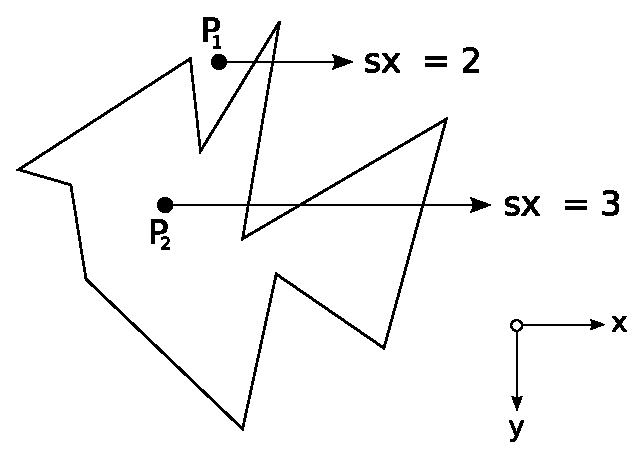
\includegraphics[]{pictures/punkt_in_polygon.eps}
    \caption{Punkt in Polygon Algorithmus}
    \label{fig:pip}
\end{figure}

Punkte werden getestest, indem man einen imagin"aren ''Strahl'' in eine
beliebige Richtung schickt und die Schnittpunkte mit den Kanten des Polygons
z"ahlt. Ist die Anzahl der Schnittpunkte gerade, so liegt der Punkt
au\ss erhalb, ist sie ungerade, so liegt der Punkt innerhalb des Polygons.

\section{Marching Cubes - Algorithmus}
\label{sec:mc_theo}

Bei dem Marching Cubes Algorithmus betrachtet man zwei benachbarte oder
"ubereinanderliegende Ebenen in einem regelm"a\ss igen Pixelraster.

\begin{figure}[htbp]
    \centering
    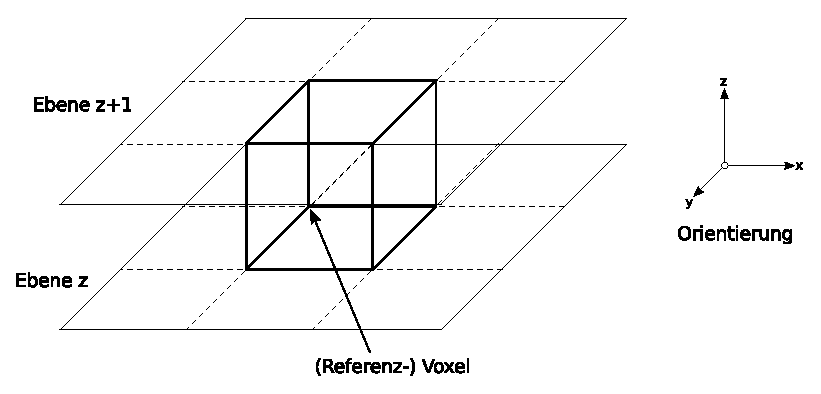
\includegraphics[]{pictures/marching_cube.eps}
    \caption{Marching Cube}
    \label{fig:mc}
\end{figure}

Nun erschafft man einen imagin"aren W"urfel, indem man acht in w"urfelform
benachbarte Punkte herausgreift und auf Schnittpunte mit einem Objekt
pr"uft.


%%%%%%%  UMSETZUNG  %%%%%%%%

\chapter{Umsetzung}

Dieses Kapitel besch"aftigt sich mit der Umsetzung und Implementierung der
vorher genannten Konzepte. Nach einer Darstellung verschiedener
L"osungsans"atze wird genauer auf den gew"ahlten Ansatz eingegangen.
Besonders herausgestellt werden der Punkt in Objekt Algorithmus sowie der
Marching Cubes Algorithmus, die den Kern dieser Arbeit darstellen.

\section{Ans"atze}

\subsection{Snow-Map}

\subsubsection{Interpretation als Lightmap}

\subsubsection{Interpretation als Light- und Displacementmap}

\subsection{Voxelrepr"asentation}

\subsubsection{Voxel}

\inputminted[linenos=true]{java}{code/SetRightNeighbor.java}

\subsubsection{1. Ansatz: F"ur beliebige Objekte}

\subsubsection{2. Ansatz: F"ur rechteckige/rasterangepasste Objekte}

Dieser Ansatz wird der in dieser Arbeit entscheidene sein.

\section{Szene auslesen}

Um nun eine Schneedecke zu simulieren muss zun"achst die vorliegende Szene
ausgelesen werden. Hierbei ist es wichtig, dass die Szene in dem sogenannten
Wavefront-Dateiformat (Dateiendung: *.obj) vorliegt. Es folgt eine
kurze Erkl"arung dieses
Dateiformats sowie die Beschreibung und Funktionsweise des Parsers.

\subsection{Wavefront-Dateiformat}

Eine Wavefront-Datei enth"alt alle f"ur die Szene relevanten Informationen,
wie Vertices, Normalen, Faces, Texturkoordinaten oder benutzte
Oberfl"achenmatrialien.
In dem folgenden Dateiausschnitt sind die f"ur diese Applikation erforderlichen
Daten beispielhaft aufgef"uhrt.

\inputminted[]{ruby}{code/cube.obj}

Die ersten beiden Zeilen k"onnen ignoriert werden, da es Kommentare sind,
deren Inhalt hier irrelevant ist.
Es sind lediglich jene Zeilen von Bedeutung, die mit ''\texttt{v}'',
''\texttt{vn}'' oder ''\texttt{f}'' beginnen.\\
Das Pr"afix ''\texttt{v}'' leitet einen Vertex ein, gefolgt von den zugeh"origen
\texttt{x}-, \texttt{y}- und \texttt{z}-Koordinaten, welche jeweils durch ein
Leerzeichen getrennt sind.
Analog dazu sind die Vertexnormalen aufgelistet, die durch das Pr"afix
''\texttt{vn}'' eingeleitet werden, mit dem Unterschied, dass die Koordinaten
keine Position, sondern eine Richtung angeben.\\
Sowohl f"ur die Vertices als auch f"ur die Normalen gilt, dass sie nur einmal
aufgelistet werden. Sollten beispielsweise an der selben Stelle mehrere
Vertices liegen, so wird dieser eine Vertex nicht mehrfach aufgef"uhrt, sondern
mehrfach verwendet (z.B. wenn mehrere Faces den selben Vertex als
Eckpunkt verwenden). Dies geschieht mit Hilfe einer impliziten Indizierung.
Jeder Vertex und jede Normale hat einen eindeutigen Index, der durch ihre
jeweilige Position in der Liste gegeben ist.\\
\\
Implizit sieht die Datei nun wie folgt aus:

\inputminted[]{ruby}{code/cube_index.obj}

Schlie\ss lich leitet das Pr"afix ''\texttt{f}'' ein Face ein. Hinter jedem
''\texttt{f}'' stehen drei durch Leerzeichen getrennte Strings in dem Format
''\texttt{<vertex\_index>//<normal\_index>}''.\\
Somit wird festgelegt, welche Vertices miteinander zu einem Face verbunden
werden m"ussen und welche Normale der jeweilige Vertex hat. Beispiel:

\inputminted[]{ruby}{face.obj}

Dieses Face besteht folglich aus dem Vertex mit dem Index 5, dem Vertex 8
und dem Vertex 7, welche in genau dieser Reihenfolge miteinander verbunden
werden. Zudem haben in diesem Fall alle drei Vertices die Normale mit dem
Index 2.


\subsection{Parser}

Mit dem oben beschriebenen Wissen "uber das vorliegende Dateiformat kann nun
ein entsprechender Parser zum Auslesen der Szene entwickelt werden. Dieser
liest die Werte ein und speichert sie zur weiteren Verarbeitung in mehreren
Arrays.\\
Dabei wird zun"achst die gesamte Datei durchgegangen um die Vorkommen der
''\texttt{v}'', ''\texttt{vn}'' und ''\texttt{f}'' zu z"ahlen und entsprechend
gro\ss e Arrays anzulegen. Diese Arrays sind:

\begin{itemize}
    \item{\textbf{vertexArray}}: Enth"alt die Vertex-Koordinaten, die
        hintereinander in das Array eingetragen werden.
    \item{\textbf{normalArray}}: Enth"alt die (Richtungs-) Koordinaten der
        Normalen, die ebenfalls hintereinander in dem Array stehen.
    \item{\textbf{faceArray}}: Enth"alt die Indizes der Vertices die zu einem
        Face verbunden werden. Ein Face besteht dabei immer aus drei Vertices.
    \item{\textbf{normalIndexArray}}: Enth"alt analog zum \texttt{faceArray} die
        Indizes der Normalen.
\end{itemize}

Nachdem die Arrays erstellt wurden, wird die Datei mit Hilfre der folgenden
\texttt{while}-Schleife erneut durchgegangen um die Arrays zu f"ullen.

\inputminted[linenos=true]{java}{code/Parser.java}

Hierbei werden jeweils die ersten zwei Zeichen jeder Zeile mit den oben
genannten Pr"afixen (hier rep"asentiert durch Konstanten) verglichen, wodurch
festgestellt wird, ob es sich um
einen Vertex, eine Normale oder ein Face handelt. Je nach "Ubereinstimmung
wird die entsprechende Methode aufgerufen, welche die Zeile durchgeht und die
einzelnen Werte in das korrekte Array eintr"agt. Dabei ist zu erw"ahnen,
dass die Methode \texttt{addFaces(String line)} beiden Index-Arrays
(\texttt{faceArray} und \texttt{normalIndexArray}) ihre Werte zuweist, da dort
immer zwei Informationen in einer Zeile stehen.

%%%%%%%% Hier evtl. noch Zugriff auf Daten erkl"aren

\section{Szene mit Voxeln f"ullen}

Nachdem die Szene nun ausgelesen werden kann und die Arrays mit den ben"otigten
Daten zur Verf"ugung stehen, soll die Szene mit Voxeln gef"ullt werden.\\
Um ein regelm"a\ss ige Voxelgitter zu erstellen muss als erstes der Platz im
Raum f"ur die Voxel bestimmt werden, das hei\ss t die Gr"o\ss e der Szene ist
zu ermitteln. Mit Hilfe des Vertex-Arrays l"asst sich nun der gr"o\ss te bzw.
kleinste in der Szene enthaltene Wert auf jeder der drei Achsen herausfinden.
Daraus lassen sich nun drei Kantenl"angen berechnen aus denen wiederum ein
Quader ermittelt werden kann, der die Szene enth"alt und mit Voxeln
aufgef"ullt wird.

Beispielhaft sei hier die Methode zur Berechnung des gr"o\ss ten
\texttt{x}-Wertes dargestellt.

\inputminted[linenos=true]{java}{code/CalculateMaxX.java}

Die Methode bekommt das gesamte Vertex-Array "ubergeben und geht alle Vertices
durch, wobei lediglich die \texttt{x}-Koordinate betrachtet wird (Zeile 7).
Es wird sich der bisher gr"o\ss te gefundene \texttt{x}-Wert gemerkt und
bei Bedarf aktualisiert und am Ende zur"uckgegeben.\\
Die Berechnung der f"unf weiteren Werte geschieht analog, mit dem Unterschied,
dass die untersuchte Koordinate des Vertex wechselt.\\
\\
Um schlie\ss lich den Quader mit Voxeln zu f"ullen wird die folgende Methode
verwendet.

\inputminted[linenos=true]{java}{code/FillScene.java}

Man geht entlang jeder Koordinatenachse die zuvor berechnete Kantenl"ange
ab und setzt einen Voxel an den entsprechenden Koordinaten. Da es sich um drei
Dimensionen handelt wird dieses Vorgehen mit drei ineinander geschachtelten
\texttt{for}-Schleifen realisiert.
Die Konstante \texttt{STEPS} stellt dabei eine Art Granularit"atsfaktor dar.
Das hei\ss t pro L"angeneinheit im Koordinatensystem werden \texttt{STEPS}
Voxel gesetzt.\\
Das Ergebnis ist in Abbildung \ref{fig:pawn_scene} zu sehen.

\begin{figure}[htbp]
    \centering
    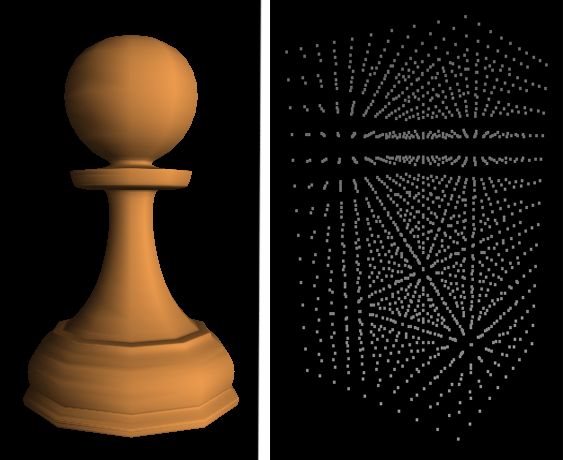
\includegraphics[width=250px]{pictures/pawn_scene.png}
    \caption{Voxelgitter}
    \label{fig:pawn_scene}
\end{figure}

Als Grundlage der Szene wurde ein Bauer eines Schachspiels beispielhaft
herangezogen (links im Bild). Die rechte Bildh"alfte stellt die ausgelesene
Szene dar in der nur die gesetzten Voxel angezeigt werden.


\section{Voxel in Objekt - Algorithmus}

In diesem Abschnitt soll die Funktionsweise des 3-dimensionalen Punkt in
Polygon Algorithmus erl"autert werden. Dieser dient dazu festzustellen, ob
ein Voxel in einem Objekt liegt, oder nicht. Mit dieser Information l"asst sich
sp"ater bestimmen an welchen Stellen der Szene Schnee fallen kann und an welchen
nicht.


\subsection{Aktive Faces berechnen}

Um etwas Rechenaufwand zu sparen, sollen nicht immer alle in der Szene
enthaltenen Faces auf Schnittpunkte mit dem aus dem Punkt in Polygon bekannten,
imagin"aren ''Strahl'' gepr"uft werden, sondern lediglich die
f"ur die jeweilige Ebene relevanten.\\ %%%%% TODO Umschreiben!!!!
Da der Algorithmus die Szene ebenenweise durchgeht m"ussen die Faces, die die
aktuelle Ebene schneiden nur ein Mal pro Ebene ermittelt werden. Das bedeutet,
dass alle Voxel in der aktuellen \texttt{x}-\texttt{y}-Ebene die selbe
\texttt{z}-Koordinate
besitzen und nur mit den gerade aktiven Faces gepr"uft werden m"ussen.

\inputminted[linenos=true]{java}{code/ActiveFaces.java}

Welches Face die betrachtete Ebene schneidet und welches nicht
bestimmt die \texttt{z}-Koordinate der drei Face-Vertices. Sind alle
\texttt{z}-Werte kleiner oder gr"o\ss er als der \texttt{z}-Wert der Ebene,
so gibt es offensichtlich keine Schnittkante. Sobald mindestens eine
\texttt{z}-Koordinate gr"o\ss er und eine andere kleiner ist als die der Ebene,
so muss es einen Schnitt geben und das Face wird zu den aktiven Faces
hinzugef"ugt. Diese Abfrage findet in dem \texttt{if}-Statement im oberen
Code-Ausschnitt statt (Zeile 8-13).

\begin{figure}[htbp]
    \centering
    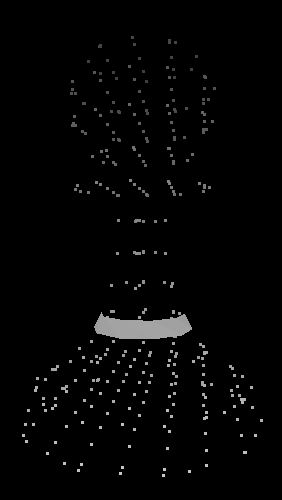
\includegraphics[width=120px]{pictures/active_faces.png}
    \caption{Aktive Faces}
    \label{fig:active_faces}
\end{figure}



\subsection{Schnittkanten der Faces mit der Ebene bestimmen}


\subsection{Punkt in Polgon - Algorithmus anwenden}

\inputminted[linenos=true]{java}{code/PunktInPolygon.java}

Ergebnis (siehe Abbildung \ref{fig:voxel_in_object}):

\begin{figure}[htbp]
    \centering
    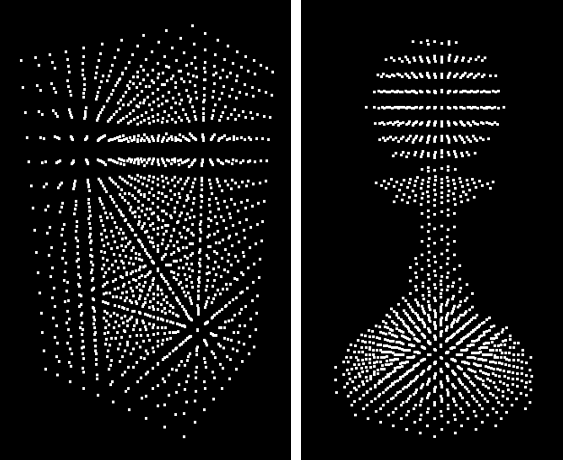
\includegraphics[width=250px]{pictures/voxel_in_object.png}
    \caption{Voxel in Objekt - Algorithmus}
    \label{fig:voxel_in_object}
\end{figure}



\section{Marching Cubes - Algorithmus}


\subsection{Imagin"aren Cube erstellen}

\inputminted[linenos=true]{java}{code/Cube.java}


\subsection{Schnittkanten mit der Ebene bestimmen}


\subsection{TriangleLookupTable}



\section{Schneedecke}



%%%%%%% REFLEXION %%%%%%%%

\chapter{Reflexion}

\section{Zusammenfassung}

\section{Fazit und Ausblick}

\newpage
Beispieltext. Siehe auch \cite{Fischer:1995, Besl:1992, Thrun:2000}.
URLs gehen auch: \cite{robocup}.


% DON'T set \bibliographystyle here -- use the documentclass option instead
\bibliography{papers}

\closing %%%%%%%%%%%%%%%%%%%%%%%%%%%%%%

\end{document}
